%TODO: add list of benchmarks, each with explanation and charactaristics.
%Add picture of complete toolflow (from C to estimates).
%Add results section,
%Add discussion on results

In order to evaluate the performance of the compiler, a set of benchmarks is used. The assembly code generated by the two compilers will be compared on `code quality' and on the number of register reads and writes it can avoid by exploiting explicit datapaths. To verify correctness of the generated code, the simulation output of the code generated by the LLVM compiler and of the code produced by the legacy compiler are compared to a reference. The references are generated using GCC\footnote{gcc.gnu.org} and the result of GCC is an executable that prints the reference output upon execution. This reference output is compared to the simulation results and if they match, the compiler can generate a correct code.

To compare the two compilers, scalar-only code is considered such that the comparison is fair. Then the auto-vectorizer is enabled for further analysis which results in more efficient code. This in turn is compared to handwritten assembly code to see how efficient the generated code truly is.

\section{Benchmarks}
The collection of benchmarks is presented in Table \ref{table:benchmarks_overview}. Originally there are more benchmarks apart from these, but they are left out because they are part of, or too similar to another benchmark. Furthermore, there is not a handwritten reference for each of these benchmarks. Namely, only \emph{binarization}, \emph{color conversion} and \emph{convolution} have vectorized assembly code references. From these references \emph{binarization} and \emph{convolution} have been handwritten by L. Waeijen, and \emph{color conversion} is vectorized by the legacy compiler using OpenCL code.

\begin{table}[H]
\caption{List of benchmarks.}
\begin{center}
\begin{tabular}{@{}l l l l@{}}
\toprule
\textbf{Benchmark} 	& \textbf{Comments} & \hspace{-30px}\textbf{Complexity}	 		\\ \hline
Addition			& Sums the individual elements of matrix $A$ and $B$.	& -- --\\
Binarization		& Converts a pixel image to a binary image. 			& --\\
Convolution		& Adds each pixel to its local neighbors, weighted by a kernel. & ++\\
DES				& A symmetric-key algorithm for encryption of data. 		& ++	\\
Histogram			& Plots the frequency distribution of a data set. 			& +\\
Matrix Multiplication	& Multiplies matrix $A$ and $B$ to form matrix $C$. 		& +\\
Matrix Transpose	& Calculates $A^T$ by reordering each row.			& +/--\\
YUV2RGB		& Color conversion to transform a YUV image to a RGB image.	& +\\
\bottomrule
\end{tabular}
\end{center}
\label{table:benchmarks_overview}
\end{table}%

\newpage

\begin{table}[t]
\caption{Summarizes which of the benchmarks have been vectorized and provides an overview of how many cycles were additionally executed because of instructions inserted by Section \ref{sec:conflicts} for both scalar- and vector-version, and how many cycles were additional executed with explicit bypassing for the legacy compiler.}
\begin{center}
\begin{tabular}{@{}l l c c c@{}}
\toprule
\textbf{Benchmark} 	& \textbf{Vectorized} & \multicolumn{3}{@{}c@{}}{\textbf{Additional cycles exec.}}	\\
				& 				& \textbf{(legacy)}	& \textbf{(scalar)} 	& \textbf{(vector)}	\\ \hline
				&				& 4st./5st.			& 4st./5st.			& 4st./5st.			\\
Addition			& Yes			& 1/2				& 0/0				& 0/0				\\
Binarization		& Yes			& 0/0				& 1/2				& 1/2				\\
Convolution		& No				& 33/32			& \ 4000/15432		& -				\\
DES				& No				& 351/367			& \ \ \ 1/770		& -				\\
Histogram			& Yes*			& 0/2				& 0/0				& 257/130\ 		\\
Matrix Multiplication	& Yes			& 0/0				& 8/2				& 1/4				\\
Matrix Transpose	& Yes*			& 0/0				& 1/0				& 1/2				\\
YUV2RGB		& Yes			&\ 0/48			& 0/0				& 1/4				\\ %TODO: determine ?
\multicolumn{5}{@{}l@{}}{\small - N/A.}\\ 
\multicolumn{5}{@{}l@{}}{\small * vectorized, but less efficient than scalar version.}\\ 
\bottomrule
\end{tabular}
\end{center}
\label{table:benchmarks_summary}
\end{table}%


%TODO: verify and rewrite this part and fill/collect future work.
The \emph{Data Encryption Standard} (DES) benchmark has not been vectorized because of irregular memory accesses. For other benchmarks e.g. \emph{histogram} and \emph{matrix transpose}, vectorization results in less efficient code. This is often caused by neighborhood network communication which is expensive for the target architecture.

%TODO: ADD PROBLEM OF CONVOLUTION VECTRIZATION, namely !! REDUCTION !!
\emph{Convolution} has not been vectorized because of an open issue with vectorized kernels that use reduction. The \emph{binarization} and \emph{YUV2RGV} benchmarks had some difficulties during vectorization because of a compilation problem when multiple set-flag and conditional move operations are present in a generated code. Problems like these and others are described in the future work section in Chapter \ref{chapter:conclusion}. In overall, the vectorized versions perform better with a speedup of ... \%. The vectorized versions are compared to scalar-only code and with the legacy compiler in Figure \ref{fig:total_domination}.


\section{Legacy Compiler Results}

\begin{figure}[b!]
\centering
\hspace*{-.12in}
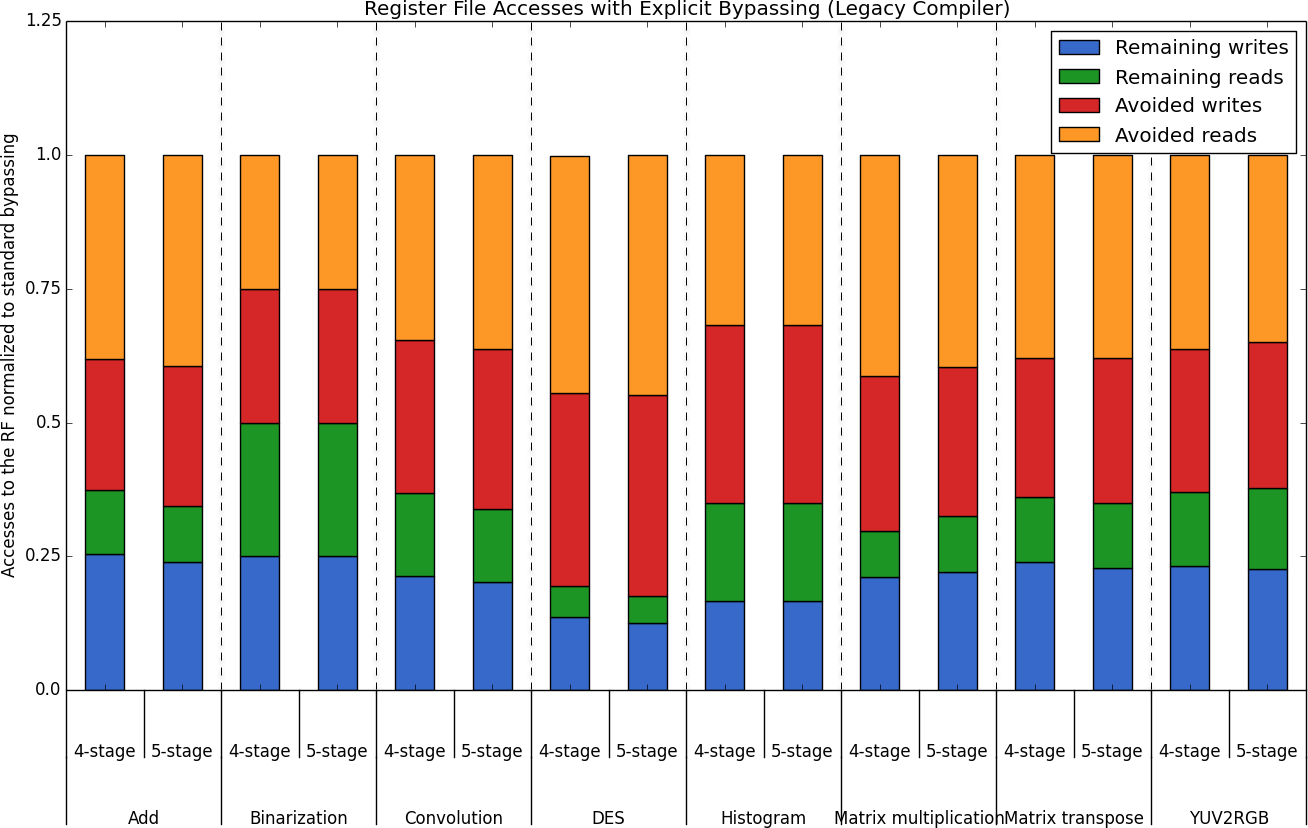
\includegraphics[width=\textwidth]{figures/stats/legacy_accesses}
\caption{Register file accesses with explicit bypassing on the legacy compiler (accesses are normalized to the total number of accesses with automatic bypassing (with an overall improvement of 70\% on writes and 56\% on reads). Note that the automatic bypass version does not avoid any write accesses, however it does avoid some read accesses.}
\label{fig:legacy_access_improvements}
\end{figure}




\section{Scalar Version Comparison}
This section compares the legacy compiler to the current compiler (Figure \ref{fig:legacy_scalar_cmp}).  

\begin{figure}[t!]
\centering
\hspace*{-.12in}
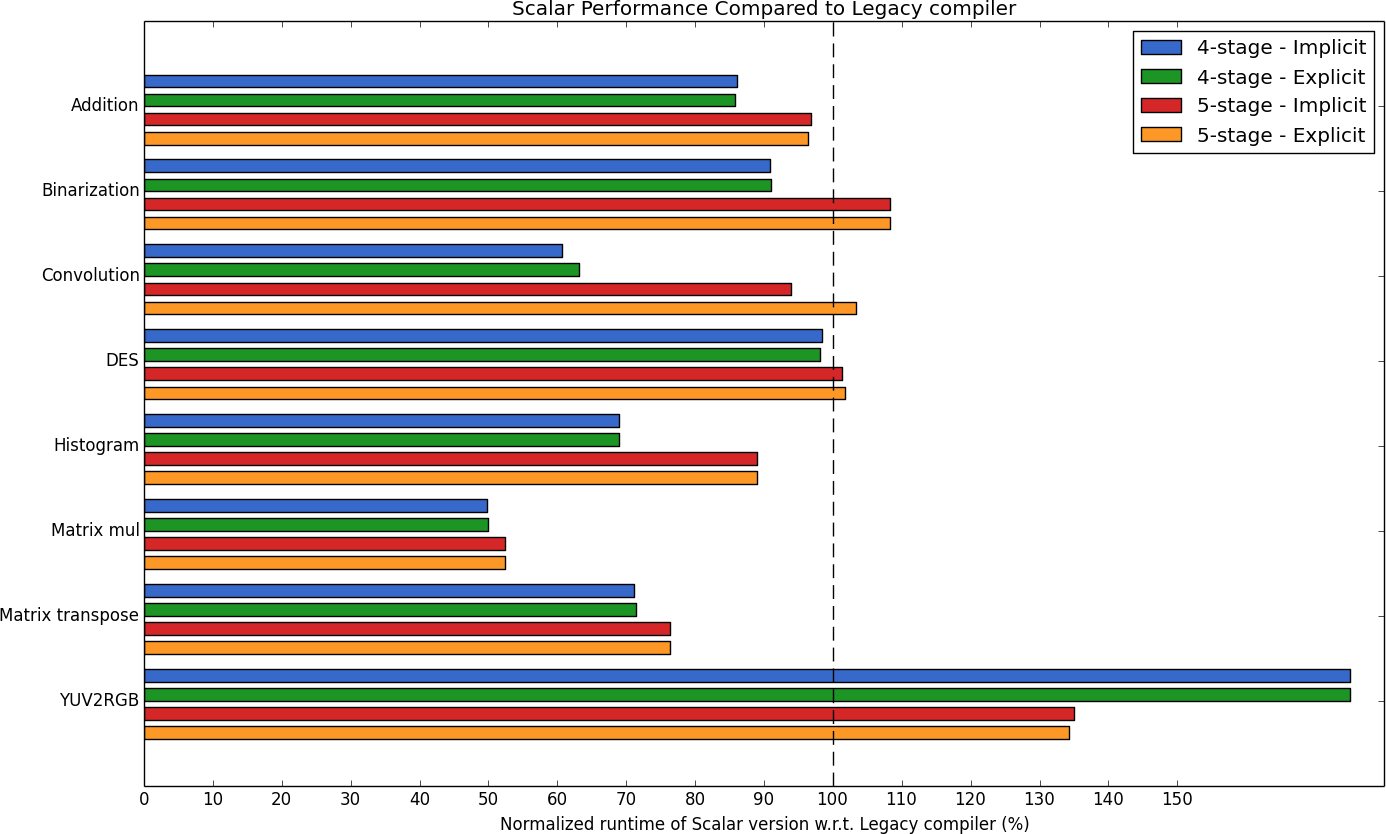
\includegraphics[width=\textwidth]{figures/stats/scalar_cycles}
%TODO: change orange to yellow and yellow to orange in picture. 
\caption{Scalar version performance comparision (cycle counts are normalized to that of the legacy compiler), with an average improvement of over 28\% in terms of cycles.}
\label{fig:legacy_scalar_cmp}
\end{figure}

%LALALALA lele

Figure \ref{fig:legacy_access_improvements} or Figure \ref{fig:legacy_write_impr} and Figure \ref{fig:legacy_read_impr}.

%%TODO rEMOVE THIS NEWPAGE
%\newpage
%%END TODO

Figure \ref{fig:scalar_improvements} shows a bar chart with how many register file accesses can be avoided by the new compiler where the accesses are normalized to automatic bypassing. The optimizations for this picture include using a scheduler optimization flag \texttt{-misched-nolimit=1} to not schedule too far, and optimization level \texttt{-O2}. The instructions are scheduled closer to their use by not buffering instructions during scheduling. The difference in the total number of cycles does not differ compared to \texttt{-O2} with no other optimization flags, but does give a overall better improvement on accesses to the RF with an average of around 60\% on register writes and 40\% on RF reads.\\

Add example \\ %Use closer to def with -misched-limit=1.



\begin{figure}[b!]
\centering
\hspace*{-.12in}
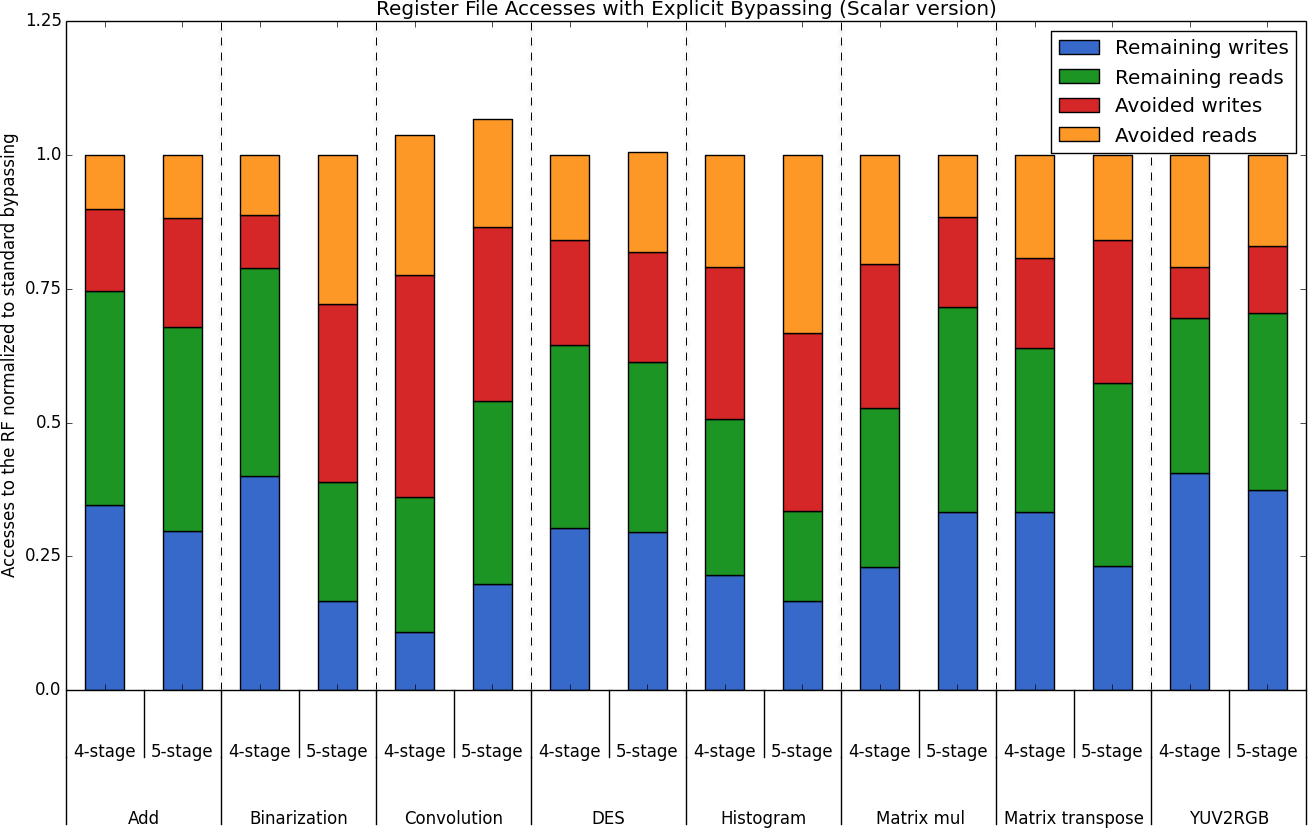
\includegraphics[width=\textwidth]{figures/stats/scalar_accesses}
%TODO: change orange to yellow and yellow to orange in picture. 
\caption{Scalar version register accesses (RF accesses are normalized to implicit bypassing), with an average improvement of over 56\% on writes and 40\% on reads.}
\label{fig:scalar_improvements}
\end{figure}



\begin{figure}[H]
\centering
\hspace*{-.12in}
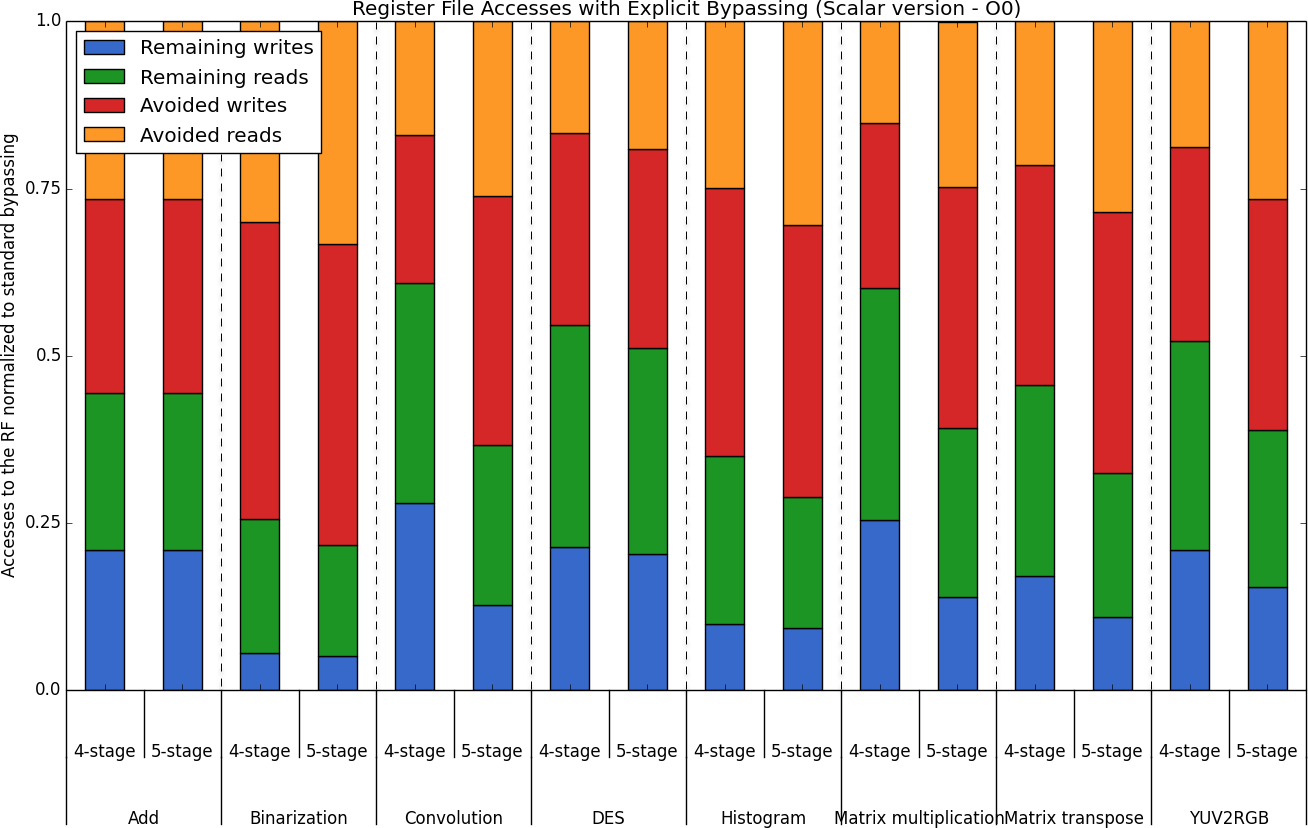
\includegraphics[width=\textwidth]{figures/stats/scalar_accesses_O0}
%TODO: change orange to yellow and yellow to orange in picture. 
\caption{Scalar version register accesses with opt-level \texttt{-O0} (RF accesses are normalized to implicit bypassing), with an average improvement of over 77\% on writes and 54\% on reads.}
\label{fig:scalar_improvements_O0}
\end{figure}

With the lowest optimization level, the savings on the register file can go up to 77\% writes and 54\% on reads on average. With such low optimization level, the total number of cycles increases rapidly with an increase in cycles of up to 6-7 times (convolution). However, for some benchmarks, e.g. histogram, it still performs quite well with only a 50\% increase in cycles, while the increase in utilization of the bypass network is significant. Figure \ref{fig:scalar_improvements_O0} shows RF accesses with explicit bypassing, the lowest optimization level and scalar-only code. A large performance lost due to such low optimization level was found for all benchmarks, except for \emph{histogram} and \emph{binarization}. For these two benchmarks which execute in around 50\% more cycles, do have a significant result by avoiding up to almost all write accesses.

%OR 

%\begin{figure}[H]
%\centering
%\subfloat[Register write improvements normalized to automatic bypassing.]{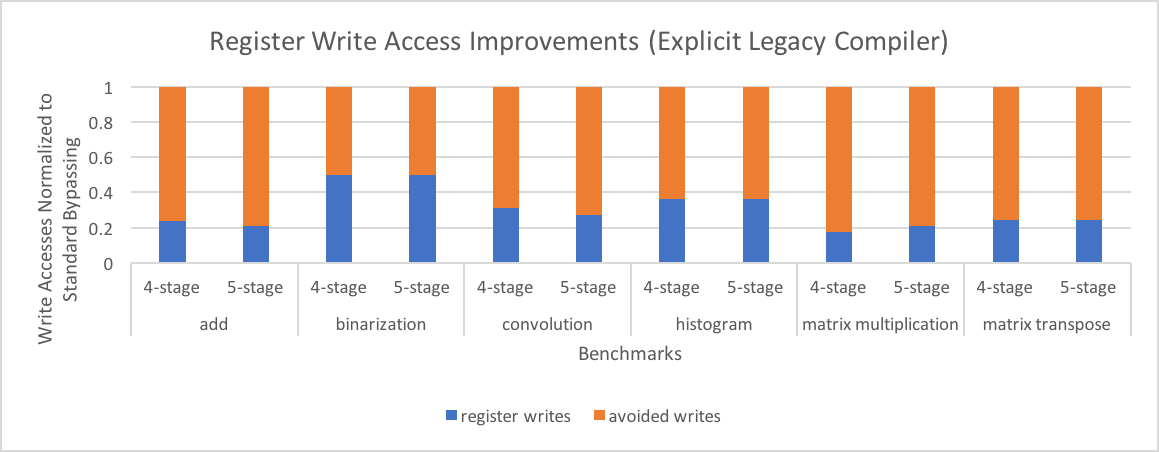
\includegraphics[width=.75\textwidth]{figures/stats/legacy_writes}%
%\label{fig:legacy_write_impr}}
%\hfil
%\subfloat[Register read improvements normalized to automatic bypassing.]{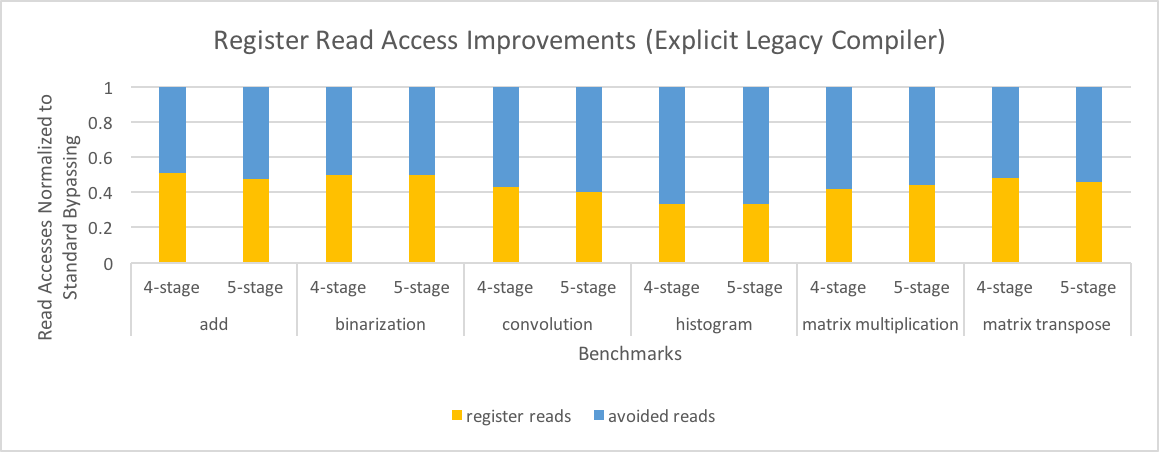
\includegraphics[width=.75\textwidth]{figures/stats/legacy_reads}%
%\label{fig:legacy_read_impr}}
%\caption{Gain in access to the bypass network, normalized to register accesses by the automatic bypass version. }
%\label{fig:legacy_access_improvements}
%\end{figure}

\section{Vector Version Comparison}

\begin{figure}[b!]
\centering
\hspace*{-.12in}
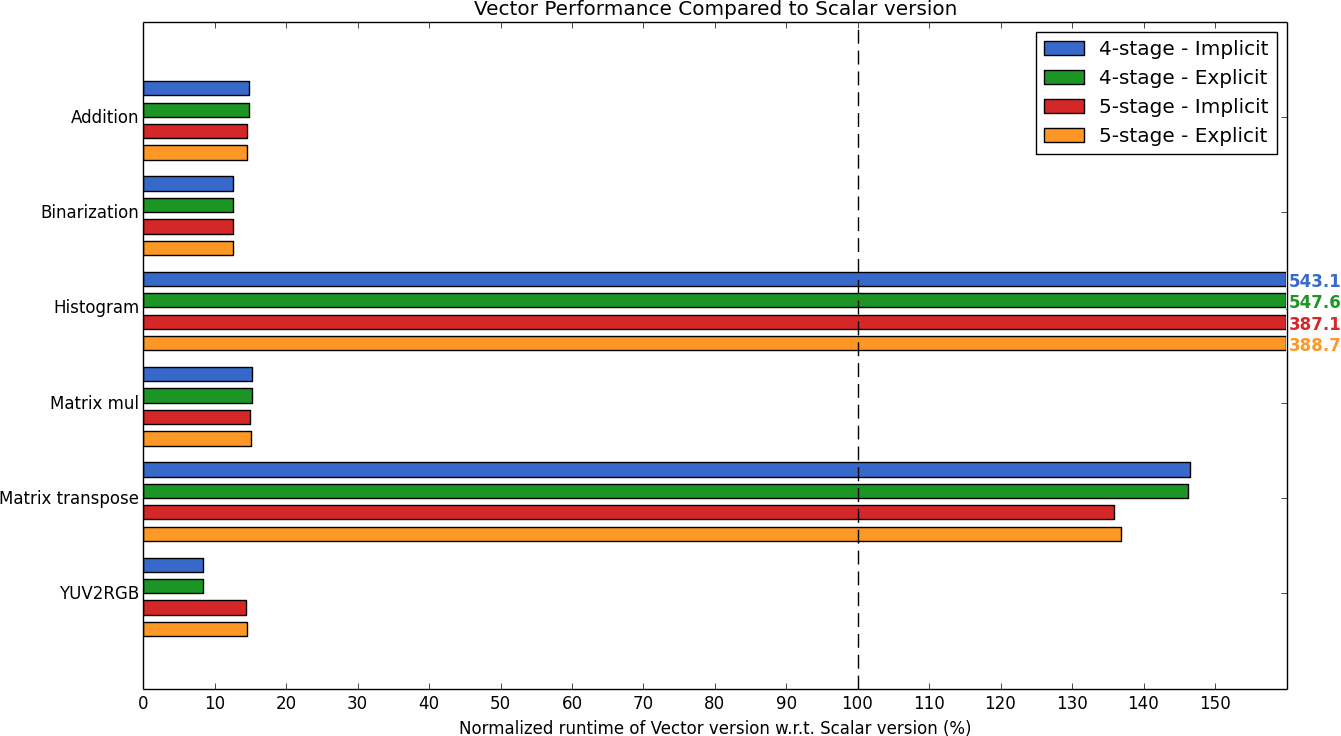
\includegraphics[width=\textwidth]{figures/stats/vector_cycles}
%TODO: change orange to yellow and yellow to orange in picture. 
\caption{Vector version performance gain (cycle counts are normalized to that of the legacy compiler), with an average improvement of 65 percent.}
\label{fig:vector_scalar_cmp}
\end{figure}


\begin{figure}[t!]
\centering
\hspace*{-.12in}
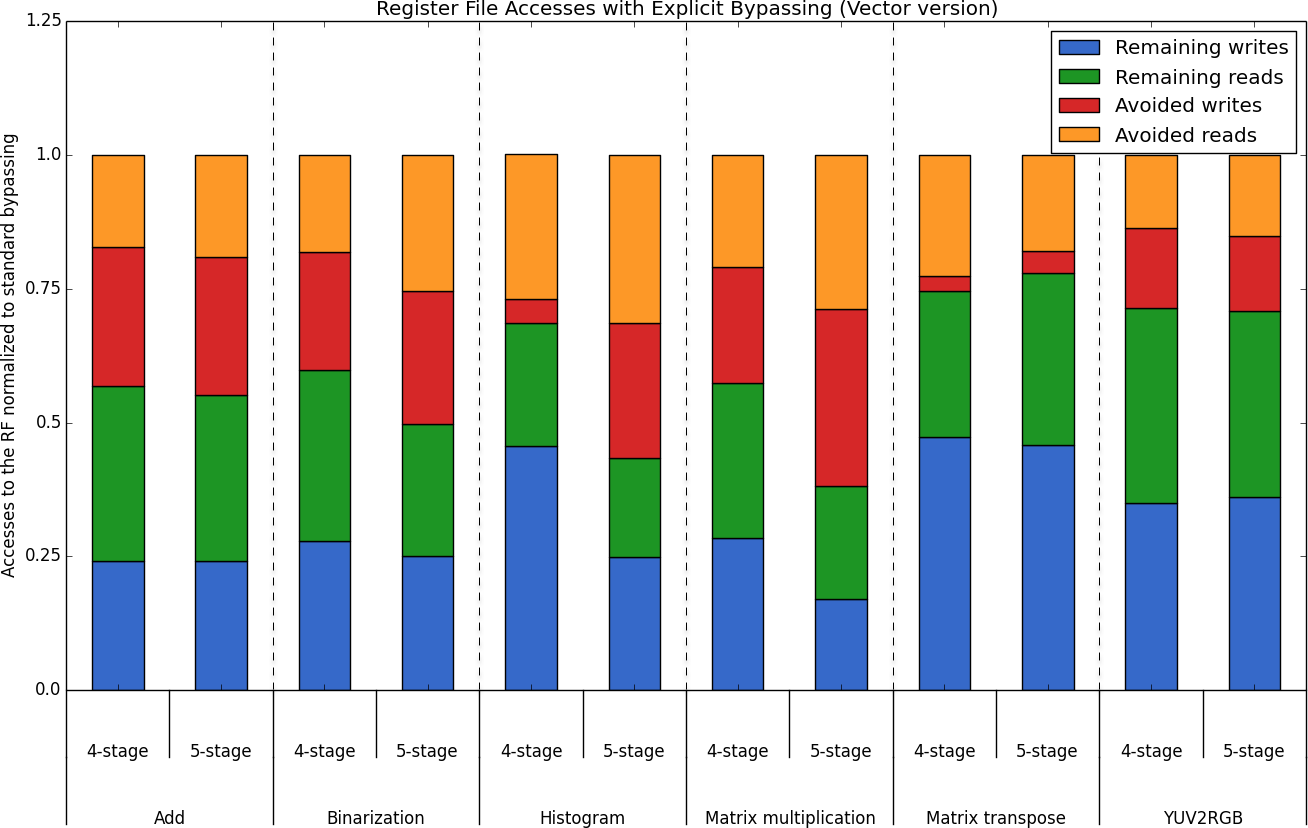
\includegraphics[width=\textwidth]{figures/stats/vec_accesses}
%TODO: change orange to yellow and yellow to orange in picture. 
\caption{RF accesses for the vector version, accesses are normalized to standard bypassing.}
\label{fig:vec_accesses}
\end{figure}


\newpage

Matrix mul benchmark, desired code. Give actual and then desired code! (that is the code below).



%TODO: discuss any inefficiencies here: 
%1: Inefficiencies by the source-level-linked, e.g. always zimm/simm in front of address to a global variable. 
%	This behaviour needs to be implemented by the standard linker too!

%2: Give one full application still needs to be done! :(
%3: discuss or at least think of a way to optimally reduce comm. using DDGs and traits


\begin{lstlisting}
A:
   addi r11, r11, -4 || v.addi r11, r11, -4
   sw   r10, r11,  0
   add  r10, r11, r0
B:
   lw   r1,  r10,  0
C:
   addi r3,  r0,   0 || v.addi r2,  r0,  16
   lw   r4,  r3,   0 || v.lw   r5,  r2,   0
   lw   r5,  r3,   1 || v.lw   r4,  r2,   1
   lw   r6,  r3,   2 || v.lw   r3,  r2,   2
   lw   r7,  r3,   3 || v.lw   r2,  r2,   3
D:
   addi r4,  r4,   0 || v.add  r6,  CP,  r0
   addi r5,  r5,   0 || v.add  r7,  CP,  r0
   nop               || v.mul  r6,  r5,  r6
   nop               || v.mul  r7,  r4,  r7
   nop               || v.add  r6,  r7,  r6
   addi r6,  r6,   0 || v.add  r7,  CP,  r0
   nop               || v.mul  r7,  r3,  r7
   addi r7,  r7,   0 || v.add  r8,  CP,  r0
   nop               || v.add  r6,  r7,  r6
   nop               || v.mul  r7,  r2,  r8
   nop               || v.add  r6,  r7,  r6
   addi r1,  r1,  -1 || v.addi r7,  r0,  32
   sfeq r1,  0       || v.sw   r6,  r7,   0
   bf   E
   nop
   j    C  
   nop
E:
   lw   r10, r11,  0
   addi r11, r11,  4 || v.addi r11, r11,  4
   jr r9
   nop
\end{lstlisting}